\documentclass[usenames,dvipsnames]{standalone}
\usepackage{tikz}
\usepackage{tikz-network}

\usepackage[T1]{fontenc}
\usepackage{libertine}
\usepackage{libertinust1math}
\usetikzlibrary{matrix, automata,arrows,positioning,calc}

\usepackage{pgfplots}

\usetikzlibrary{patterns.meta,decorations.pathmorphing}

\begin{document}
	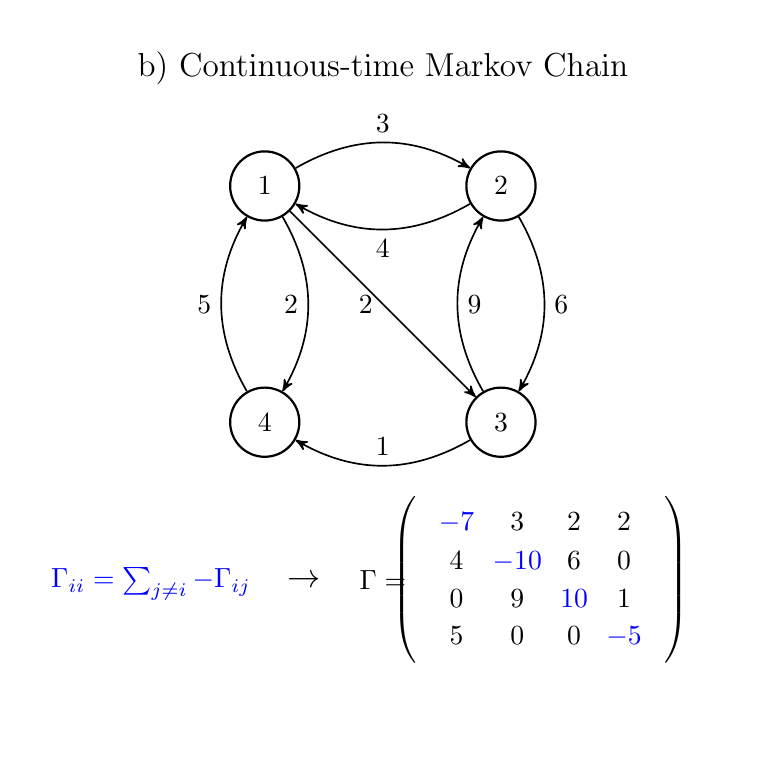
\begin{tikzpicture}[->, >=stealth', auto, semithick, node distance=3cm]
		
		% Example of discrete time Markov Chain
		\draw[white] rectangle(9, 9);
		\draw[black] node (title) at (4.5, 8.5) {\large b) Continuous-time Markov Chain};
		
		\tikzstyle{every state}=[fill=white,draw=black,thick,text=black,scale=1]
		\node[state]    (1) at (3, 7)     {$1$};
		\node[state]    (2)[right of=1]   {$2$};
		\node[state]    (4)[below of=1]   {$4$};
		\node[state]    (3)[below of=2]   {$3$};
		
		%		\path (1) edge[bend left]     	node{$p_{12}$} (2);
		%		\path (1) edge[loop left]     	node{$p_{11}$} (1);
		%		\path (2) edge[bend left]     	node{$p_{21}$} (1);
		%		\path (2) edge[loop right]     	node{$p_{22}$} (2);
		%		\path (2) edge[bend left]     	node{$p_{23}$} (3);
		%		\path (1) edge[bend right, left]node{$p_{14}$} (4);
		%		\path (4) edge[bend right, left]node{$p_{41}$} (1);
		%		\path (4) edge[loop left]     	node{$p_{44}$} (4);
		%		\path (1) edge[midway, below] 	node{$p_{13}$} (3);
		%		\path (3) edge[bend left, right]node{$p_{32}$} (2);
		%		\path (3) edge[bend right] 		node{$p_{34}$} (4);
		%		
		
		\path (1) edge[bend left]     	node{$3$} (2);
		\path (2) edge[bend left]     	node{$4$} (1);
		\path (2) edge[bend left]     	node{$6$} (3);
		\path (1) edge[bend left, left]node{$2$} (4);
		\path (4) edge[bend left, left]node{$5$} (1);
		\path (1) edge[midway, left] 	node{$2$} (3);
		\path (3) edge[bend left, right]node{$9$} (2);
		\path (3) edge[bend left, above] 		node{$1$} (4);
		
		
		% The corresponding matrix P
		\matrix [matrix of math nodes, left delimiter=(,right delimiter=)](P) at (6.5, 2){ 
			\color{blue}-7 & 3 &  2 &  2\\
			4 & \color{blue}-10 &  6 &  0  \\  
			0 & 9 &  \color{blue}10 &  1\\
			5 & 0 &  0 &  \color{blue}-5\\
		};	
		
		\draw node (p) at (4.5, 2) {$\Gamma = $};

		\draw node (p) at (2, 1.95) {\color{blue} $\Gamma_{ii} = \sum_{j\neq i} -\Gamma_{ij}$  \quad \color{black} \large $\rightarrow$};
		
		
	\end{tikzpicture}
\end{document}